\documentclass{article}
\usepackage{physics}
\usepackage{graphicx}
\usepackage{caption}
\usepackage{amsmath}
\usepackage{bm}
\usepackage{framed}
\usepackage{authblk}
\usepackage{empheq}
\usepackage{amsfonts}
\usepackage{esint}
\usepackage[makeroom]{cancel}
\usepackage{dsfont}
\usepackage{centernot}
\usepackage{mathtools}
\usepackage{bigints}
\usepackage{amsthm}
\theoremstyle{definition}
\newtheorem{defn}{Definition}[section]
\newtheorem{prop}{Proposition}[section]
\newtheorem{rmk}{Remark}[section]
\newtheorem{thm}{Theorem}[section]
\newtheorem{exmp}{Example}[section]
\newtheorem{prob}{Problem}[section]
\newtheorem{sln}{Solution}[section]
\newtheorem*{prob*}{Problem}
\newtheorem{exer}{Exercise}[section]
\newtheorem*{exer*}{Exercise}
\newtheorem*{sln*}{Solution}
\usepackage{empheq}
\usepackage{tensor}
\usepackage{xcolor}
%\definecolor{colby}{rgb}{0.0, 0.0, 0.5}
\definecolor{MIT}{RGB}{163, 31, 52}
\usepackage[pdftex]{hyperref}
%\hypersetup{colorlinks,urlcolor=colby}
\hypersetup{colorlinks,linkcolor={MIT},citecolor={MIT},urlcolor={MIT}}  



\newcommand*\widefbox[1]{\fbox{\hspace{2em}#1\hspace{2em}}}

\newcommand{\p}{\partial}
\newcommand{\R}{\mathbb{R}}
\newcommand{\C}{\mathbb{C}}
\newcommand{\lag}{\mathcal{L}}
\newcommand{\nn}{\nonumber}
\newcommand{\ham}{\mathcal{H}}
\newcommand{\M}{\mathcal{M}}
\newcommand{\I}{\mathcal{I}}
\newcommand{\K}{\mathcal{K}}
\newcommand{\F}{\mathcal{F}}
\newcommand{\w}{\omega}
\newcommand{\lam}{\lambda}
\newcommand{\al}{\alpha}
\newcommand{\be}{\beta}
\newcommand{\x}{\xi}

\newcommand{\G}{\mathcal{G}}

\newcommand{\f}[2]{\frac{#1}{#2}}

\newcommand{\ift}{\infty}

\newcommand{\lp}{\left(}
\newcommand{\rp}{\right)}

\newcommand{\lb}{\left[}
\newcommand{\rb}{\right]}

\newcommand{\lc}{\left\{}
\newcommand{\rc}{\right\}}


\newcommand{\V}{\mathbf{V}}
\newcommand{\U}{\mathcal{U}}
\newcommand{\Id}{\mathcal{I}}
\newcommand{\D}{\mathcal{D}}
\newcommand{\Z}{\mathcal{Z}}

%\setcounter{chapter}{-1}






\usepackage{subfig}
\usepackage{listings}
\captionsetup[lstlisting]{margin=0cm,format=hang,font=small,format=plain,labelfont={bf,up},textfont={it}}
\renewcommand*{\lstlistingname}{Code \textcolor{violet}{\textsl{Mathematica}}}
\definecolor{gris245}{RGB}{245,245,245}
\definecolor{olive}{RGB}{50,140,50}
\definecolor{brun}{RGB}{175,100,80}

%\hypersetup{colorlinks,urlcolor=colby}
\lstset{
	tabsize=4,
	frame=single,
	language=mathematica,
	basicstyle=\scriptsize\ttfamily,
	keywordstyle=\color{black},
	backgroundcolor=\color{gris245},
	commentstyle=\color{gray},
	showstringspaces=false,
	emph={
		r1,
		r2,
		epsilon,epsilon_,
		Newton,Newton_
	},emphstyle={\color{olive}},
	emph={[2]
		L,
		CouleurCourbe,
		PotentielEffectif,
		IdCourbe,
		Courbe
	},emphstyle={[2]\color{blue}},
	emph={[3]r,r_,n,n_},emphstyle={[3]\color{magenta}}
}


\begin{document}
	

\begin{center}
	\Large{Some Magnetic Traps for Neutral Atoms \\
	\& The Majorana Spin-flip for $J=1/2$.}
\end{center}	
	
\begin{center}
	\large{Huan Q. Bui}
\end{center}

\begin{center}
	\today
\end{center}



\section{Notebook}
The Mathematica notebook which contains all calculations and sketches can be downloaded via this \href{}{link}. 

\section{Quadrupole trap (anti-Helmholtz)}



\subsection{Calculation}


In this configuration, there are two coils of radius $a$ placed at distance $2b$ apart. Running through the coils are equal and opposite currents $I$ and $-I$, respectively. Here, we set $I = NI_0$ where $N$ is the number of coils and $I_0$ is the current going through each coil (or equivalently through all the coils).

\begin{figure}[!htb]
	\centering
	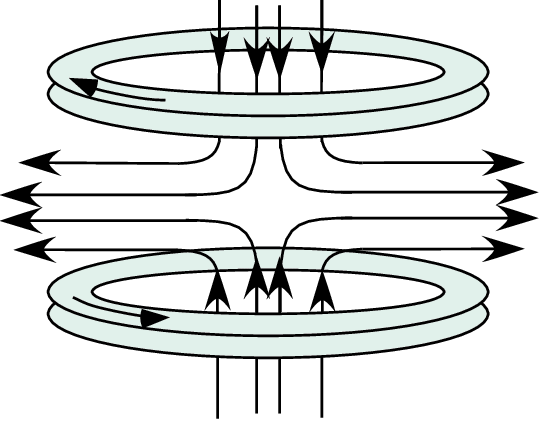
\includegraphics[width=0.6\textwidth]{antiHelmholtz.png}
	\caption{From \cite{maruyama2003optical}}
\end{figure}

To calculate the magnetic field for one coil, we can use Biot-Savart law because the current is constant. We will integrate along the closed loop $C$ defined by the coil. The relative position between the point $\mathbf{r}$ and the point $\vec{l}$ on the wire is given by $\vec{r}' = \vec{r} - \vec{l}$
\begin{equation*}
\vec{B}(\vec{r}) = \f{\mu_0 I}{4\pi} \int_C \f{d\vec{l} \times \vec{r}'}{ |{\vec{r}'}|^3} = \f{\mu_0 I}{4\pi} \int_C \f{d\vec{l} \times (\vec{r} - \vec{l})}{|{\vec{r} - \vec{l}}|^3}.  
\end{equation*}
We now make the approximation $|\vec{r}| \ll \vec{l}$ (i.e., we're interested in points far from the coil). With this we have the following expansion
\begin{equation*}
\f{1}{|\vec{r} - \vec{l}|^3} \approx \f{1}{|\vec{l}|^3} + \f{3 \vec{r}\cdot \vec{l}}{|\vec{l}|^5} + \dots
\end{equation*}
Plugging this back in for $\vec{B}(\vec{r})$ we find 
\begin{equation*}
\vec{B}(\vec{r}) \approx \f{\mu_0 I}{4\pi}\int_C d\vec{l}\times \f{\vec{r} - \vec{l}}{|\vec{l}|^3} + \f{3\mu_0 I}{4\pi} \int_C d\vec{l} \times (\vec{r} - \vec{l}) \f{\vec{r}\cdot \vec{l}}{|\vec{l}|^5}.
\end{equation*}
Suppose that the center of the coil is at $+d$ from the $XY$ plane. Going into cylindrical coordinates, we have
\begin{equation*}
\vec{l} = a\cos\theta\hat{x} + a\sin\theta\hat{y} + d\hat{z}
\end{equation*}
from which we find 
\begin{equation*}
d\vec{l} = -a\sin\theta d\theta\hat{x} + a\cos\theta d\theta \hat{y}
\end{equation*}
So, we have
\begin{equation*}
d\vec{l} \times (\vec{r} - \vec{l}) = (-a\sin\theta, a\cos\theta,0)\times(x-a\cos\theta,y-a\sin\theta,z-d)
\end{equation*}
and 
\begin{equation*}
\vec{r}\cdot \vec{l} = xa\cos\theta + ya\sin\theta + za.
\end{equation*}
So, we have
\begin{equation*}
\f{\mu_0 I}{4\pi}\int_C d\vec{l}\times \f{\vec{r} - \vec{l}}{|\vec{l}|^3} = \f{\mu_0 I }{4\pi} \f{2a^2 \pi}{(d^2 + a^2)^{3/2}} \hat{z} = \f{\mu_0 I a^2}{2(d^2 + a^2)^{3/2}} \hat{z}.
\end{equation*}
and 
\begin{align*}
&\f{3\mu_0 I }{4\pi}\int_C d\vec{l}\times (\vec{r} - \vec{l}) \f{\vec{r}\cdot \vec{l}}{|\vec{l}|^5}\\ 
=\,\, &\f{3\mu_0 Ia^2}{4(d^2+a^2)^{5/2}} \left(- x(d-z)\hat{x}  - y (d-z)\hat{y} -  (x^2 + y^2 - 2dz)\hat{z}\right).
\end{align*}
Keeping only the linear terms and combining everything, we find the total field:
\begin{align*}
\vec{B}(\vec{r}) &= \f{\mu_0 I a^2}{2(d^2 + a^2)^{3/2}} \hat{z} + \f{3\mu_0 Ia^2}{4(d^2+a^2)^{5/2}} \left(- xd\hat{x}  -  y d\hat{y} - 2dz\hat{z}\right)\\
&= \f{\mu_0 I a^2}{2(d^2 + a^2)^{3/2}} \hat{z} + \f{3\mu_0 Ia^2 d}{2(d^2+a^2)^{5/2}} \left(- \f{x}{2}\hat{x}  -  \f{y}{2}\hat{y} - z\hat{z}\right).
\end{align*}






In the anti-Helmholtz configuration, we have two coils of radius $a$ placed a distance $2b$ apart from each other. When summing the two fields to get the total field, the first term cancels. So we get
\begin{equation*}
\vec{B}_\text{tot}(\vec{r}) = \vec{B}_{+b}(\vec{r}) + \vec{B}_{-b}(\vec{r}) = -\f{3\mu_0 I a^2 b}{2(a^2 + b^2)^{5/2}}\left( x,y,-2z \right) \equiv B_0 (x,y,-2z).
\end{equation*}
The field strength is given by 
\begin{equation*}
\abs{B(\vec{r})} = B_0 \sqrt{x^2 + y^2 + 4z^2}.
\end{equation*}



\subsection{Trap parameters}

\subsection{Simulation}




\newpage

\section{TOP trap}


\subsection{Calculation}

As will be discussed later, the quadrupole or anti-Helmholtz trap suffers from the ``Majorna spin-flip problem'' which occurs due to the presence of a zero-magnetic field point in the trap. To overcome this issue, one can add a rotating magnetic field to the existing anti-Helmholtz field so that the time-averaged magnetic field no longer has a zero at the center. This trick gives us the TOP (time orbiting potential) trap. The total field is given by 
\begin{equation*}
\vec{B}(\vec{r},t) = \vec{B}_\text{quad}(\vec{r}) + \vec{B}_b(\vec{r}) = B_0 (x,y,-2z) + B_b(\cos\Omega t, \sin\Omega t,0),
\end{equation*} 
where $\Omega$ is the angular frequency of the rotating field. \\


The field strength is given by 
\begin{equation*}
B(\vec{r},t) = \sqrt{(B_0 x + B_b\cos\Omega t)^2 + (B_0 y + B_b\sin\Omega t)^2 + 4 B_0^2 z^2 }
\end{equation*}

\begin{figure}[!htb]
	\centering
	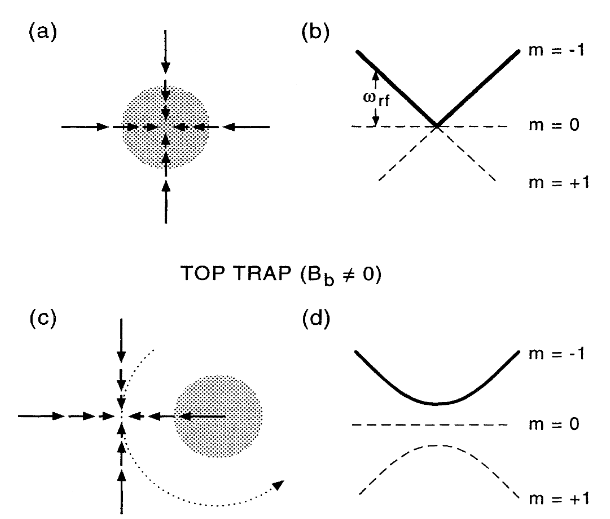
\includegraphics[width=0.6\textwidth]{TOP_trap.png}
	\caption{From \cite{PhysRevLett.74.3352}}
\end{figure}

For this trap to work $\Omega$ can't be too small or too large. $\Omega$ must be larger than the oscillation frequency of the trapped particles (which is on the order of $100$ Hz) so that the particles feel an effective time-averaged magnetic field. $\Omega$ should also be smaller than the frequency associated with the transition between two adjacent internal quantum states (which is on the order of $1$ MHz) in order to prevent particle losses due to Majorana spin-flips. \\


We are interested in dynamics near the center of the trap, so we can make the approximation $r = \sqrt{x^2 + y^2 + z^2} \ll a$, under which 
\begin{equation*}
B(\vec{r},t)\approx B_b + \f{B_0^2}{2B_b^2} (x^2 + y^2 + 4z^2) + \f{B_0}{B_b}(x\cos\Omega t+ y\sin\Omega t) - \f{B_0^2}{2B_b^2}(x\cos\Omega t + y\sin\Omega t)^2.
\end{equation*}
The time-averaged magnetic field strength is thus, by inspection,
\begin{align*}
\langle B \rangle 
&= B_b  + \f{B_0^2}{2B_b^2} (x^2 + y^2 + 4z^2) - \f{B_0^2}{2B_b^2}\lp \f{x^2}{2} + \f{y^2}{2}\rp\\ &= B_b + \f{B_0^2}{4B_b}(x^2 + y^2 + 8z^2).
\end{align*}


\subsection{Trap parameters}

\subsection{Simulation}


\section{Ioffe-Pritchard traps}



\subsection{Calculation}


There are many variants of the IP trap, the simplest being one with two coils in the anti-Helmholtz configuration and four wires in the $z$-direction. The four wires are suited at the corners of a square, with the currents flowing along adjacent wires being of opposite sign. A generalization of the IP trap is often called the ``all coils Ioffe-Pritchard trap.'' The all-coil trap consists of the following set of coils:
\begin{itemize}
	\item Big Ioffe Coils (BI), anti-Helmholtz, along $z$
	\item Small Ioffe Coils (SI), anti-Helmholtz, along $x$
	\item Pinch coils (PI), Helmholtz, along $y$
	\item Compensation coils (CO), Helmholtz, along $y$, opposite current to SI.
\end{itemize}

Let us revisit the calculation we've done for Helmholtz and anti-Helmholtz coils, but now we will expand to higher orders (still assuming that $\vec{r}$ is near the origin). In particular, we will use
\begin{equation*}
\f{1}{|\vec{r} - \vec{l}|^3} \approx \f{1}{|\vec{l}|^3} + \f{3 \vec{r}\cdot \vec{l}}{|\vec{l}|^5} + \f{15}{2}\f{(\vec{r}\cdot\vec{l})^2}{|\vec{l}|^7} + \f{35}{2} \f{(\vec{r}\cdot \vec{l})^3}{|\vec{l}|^9}.
\end{equation*}
The expansion can be obtained by following 
Eq. 3.88 of \cite{griffiths2005introduction}. For a single coil with current $I$ placed a vertical distance $+d$ from the origin, we find the factor $|\vec{l}| = \sqrt{a^2 + d^2}$ to be constant. The field, order-by-order to third order, is thus  
\begin{equation*}
B^{(0)}(\vec{r}) = \f{\mu_0 I}{4\pi |\vec{l}|^3}\int_C d\vec{l}\times (\vec{r} - \vec{l}) = \f{1}{2}\f{\mu_0 I a^2}{(a^2 + d^2)^{3/2}} \hat{z} \equiv \f{1}{2}\mathbb{F}\hat{z}
\end{equation*}
\begin{align*}
B^{(1)}(\vec{r}) &= \f{3\mu_0 I}{4\pi |\vec{l}|^5}\int_C d\vec{l}\times (\vec{r} - \vec{l}) \vec{r}\cdot \vec{l}\\
&=\f{3\mu_0 Ia^2}{4(d^2+a^2)^{5/2}} \left(- x(d-z)\hat{x}  - y (d-z)\hat{y} -  (x^2 + y^2 - 2dz)\hat{z}\right)\\
&\approx \f{3\mu_0 Ia^2 d}{2(d^2+a^2)^{5/2}} \left(-\f{x}{2}\hat{x}  - \f{y}{2}\hat{y} + z\hat{z}\right)\\
&\equiv \mathbb{G}\left(-\f{x}{2}\hat{x}  - \f{y}{2}\hat{y} + z\hat{z}\right)
\end{align*}
\begin{align*}
B^{(2)}(\vec{r}) 
&= \f{15\mu_0 I}{8\pi |\vec{l}|^7}\int_C d\vec{l}\times (\vec{r} - \vec{l}) (\vec{r}\cdot \vec{l})^2\\
&= 
\end{align*}
\begin{equation*}
B^{(3)}(\vec{r}) = \f{35\mu_0 I}{8\pi |\vec{l}|^9}\int_C d\vec{l}\times (\vec{r} - \vec{l}) (\vec{r}\cdot \vec{l})^3 = 
\end{equation*}

\subsection{Trap parameters}

\subsection{Simulation}




\begin{figure}[!htb]
	\centering
	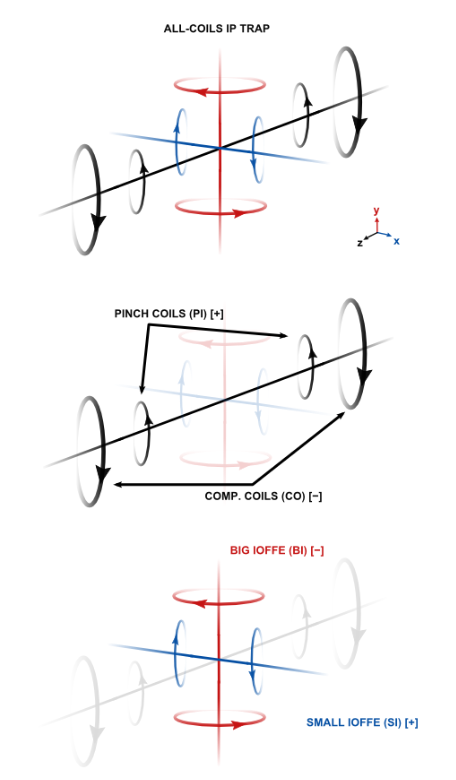
\includegraphics[width=0.75\textwidth]{all-coils.png}
	\caption{From \cite{allcoil}}
\end{figure}



\typeout{}
\bibliography{Bui_MagTrap.bib} 
\bibliographystyle{unsrt}	

\end{document}